\documentclass[11pt]{article}

\usepackage[a4paper,margin=2.4cm]{geometry}
\usepackage{amsmath}
\usepackage{booktabs}
\usepackage{graphicx}
\usepackage[numbers,sort&compress]{natbib}
\usepackage{xcolor}
\usepackage[hidelinks]{hyperref}

\newcommand{\impmodel}{IMP--MiT-B3 U-Net}
\newcommand{\cleanv}{Clean-v3}

\title{Evidence-Bounded Comparison of MiT-B3 U-Net and nnU-Net for Skin Lesion Segmentation}
\author{Nguyễn Trần Minh Quân \and Nguyễn Đức Lân}
\date{July 2026}

\begin{document}
\maketitle

\begin{abstract}
Reliable dermoscopic lesion segmentation requires more than a high overlap score: dataset leakage, image-quality variation, boundary errors, and post-hoc model selection can each invalidate an apparently strong result. We report an evidence-bounded comparison built after auditing the IMP project's data lineage. The leakage-audited \cleanv{} manifest contains 2,869 images split into 2,008 training, 431 validation, and 430 sealed test images with no detected cross-split identity-group overlap. On the already-opened, adaptively used \cleanv{} development-validation partition, the project's preprocessing-aware MiT-B3 U-Net control obtained robust Dice 0.8959 and boundary F1 0.4145, while a raw-RGB nnU-Net v2 model obtained robust Dice 0.9019 and boundary F1 0.4369. These are selection-optimistic, single-run point estimates under an older geometry contract; the protected test partition was not opened, so they do not establish statistical superiority or state of the art. We additionally analyze a controlled three-seed train-screen experiment in which a saliency-constrained active-contour mask was supplied as a fourth channel. Contrary to the motivating hypothesis, the contour channel changed seed-and-view-averaged robust Dice by $-0.0313$ (95\% split-group cluster-bootstrap confidence interval $[-0.0491,-0.0156]$, conditional on the three selected seeds). The boundary-F1 change was $-0.0147$ ($[-0.0308,0.0010]$). The result rejects this implementation before protected evaluation but does not quantify uncertainty over seed selection. The report demonstrates a useful outcome even without a positive model claim: leakage-aware evidence classification, strong-baseline comparison, and documentation of a negative ablation can prevent an internal benchmark from becoming an unsupported leaderboard claim.
\end{abstract}

\noindent\textbf{Keywords:} skin lesion segmentation; dermoscopy; nnU-Net; MiT-B3; data leakage; robustness; active contour; negative results

\section{Introduction}

Automatic segmentation of pigmented skin lesions supports quantitative image analysis, follow-up, and computer-aided research. The task remains difficult because lesion borders can be faint, hairs and acquisition artifacts can occlude the target, and illumination, contrast, blur, noise, and compression vary across sources. Region-overlap metrics can also hide clinically visible boundary failures. A useful benchmark must therefore control data identity, preprocessing, model selection, metric geometry, and access to protected partitions rather than treating a single Dice value as sufficient evidence.

This report was motivated by an audit of a long-running experimental repository. An earlier Clean-v2 benchmark contained three patient identifiers and 13 rows that crossed split boundaries. Those experiments included a broad panel---a preprocessing-aware MiT-B3 model, an architecture-matched vanilla model, EGE-UNet, and nnU-Net---and produced apparently competitive test values. Patient overlap, however, invalidates an independent patient-level generalization interpretation. Following the principle that leakage must be treated as a scientific design defect rather than a cosmetic limitation \citep{kapoor2023leakage}, the affected results are retained only as historical evidence.

The repaired \cleanv{} protocol separates evidence into protected validation, train-screen, protected test, external audit, and contaminated legacy classes. This distinction changes the research question. Rather than asking whether one internal number is ``best,'' we ask:

\begin{quote}
Under a leakage-audited dermoscopic lesion segmentation workflow, how do a preprocessing-aware MiT-B3 U-Net pipeline and nnU-Net v2 trade region overlap against boundary quality, and does an explicit saliency-constrained contour channel improve a matched MiT-B3 control?
\end{quote}

Two hypotheses follow. First, the self-configuring nnU-Net pipeline should improve robust validation overlap and boundary quality relative to the current IMP control. Second, an explicit contour channel should improve boundary localization without materially reducing Dice. The available evidence is asymmetric: the architecture comparison consists of single-run validation point estimates under a known older geometry contract, whereas the contour-channel experiment is a paired, three-seed, train-screen ablation with cluster-bootstrap intervals. The claims are therefore separated rather than collapsed into one ranking.

The contributions of this report are:

\begin{enumerate}
    \item an evidence hierarchy that prevents contaminated, train-screen, validation, and protected-test results from being ranked as if they were interchangeable;
    \item a bounded \cleanv{} validation comparison between the IMP MiT-B3 U-Net control and nnU-Net v2 using overlap and boundary metrics;
    \item a controlled negative ablation showing that the tested Loop206 contour channel materially reduces robust Dice across three paired seeds; and
    \item a reproducibility and demonstration design in which paper tables and website labels are generated from the same hash-bound evidence registry.
\end{enumerate}

No contribution is presented as a protected-test result, a statistically significant architecture comparison, a clinical system, or a state-of-the-art claim.

\section{Related Work}

\subsection{Biomedical segmentation architectures}

U-Net established the encoder--decoder template with skip connections that remains central to biomedical segmentation \citep{unet2015}. Attention U-Net and UNet++ subsequently introduced attention gating and nested skip pathways \citep{attentionunet2018,unetplusplus2018}. Transformer encoders provide a complementary mechanism for multiscale contextual modeling. SegFormer introduced a hierarchical Mix Transformer (MiT) encoder and a lightweight all-MLP decoder for semantic segmentation \citep{segformer2021}. The IMP implementation uses a MiT-B3 encoder inside the U-Net decoder supplied by \texttt{segmentation-models-pytorch}; it is therefore not an exact reproduction of the original SegFormer decoder. We retain the historical project label in artifact identifiers but use ``MiT-B3 U-Net'' when describing the implemented architecture.

nnU-Net takes a different position: it treats preprocessing, architecture configuration, training, inference, and postprocessing as an integrated self-configuring pipeline \citep{nnunet2021}. This makes nnU-Net a stronger comparator than a weak manually configured U-Net. Lesion-specific systems such as EGE-UNet target efficient multiscale aggregation \citep{egeunet2023}, while DermoSegDiff investigates boundary-aware diffusion modeling \citep{dermosegdiff2023}. These methods motivate broader architecture panels, but only models evaluated under a common leakage-safe protocol can support direct ranking in this report.

\subsection{Appearance normalization and robustness}

Dermoscopy pipelines commonly attempt to normalize local contrast and color variation. Contrast-limited adaptive histogram equalization enhances local luminance contrast while limiting amplification \citep{zuiderveld1994clahe}. Shades-of-Gray color constancy estimates scene illumination through a Minkowski-norm generalization of Gray World \citep{finlayson2004shades}. Such operations can improve visibility but can also suppress weak boundary evidence or amplify noise. The relevant causal question is not whether a processed image appears clearer, but whether a fixed operation improves a matched model under controlled corruptions.

\subsection{Saliency and active contours}

Regional saliency methods use color, texture, spatial layout, and background connectivity to estimate lesion support. Supervised saliency and background-detection approaches have been studied directly for dermoscopic segmentation \citep{jahanifar2019saliency,ahn2017background}. Active-contour and level-set methods then refine a coarse support using image gradients and shape evolution; distance-regularized level-set evolution is a representative formulation \citep{li2010drlse}. Loop206 combines a learned regional saliency map with a morphological geodesic active contour. It is paper-inspired engineering, not an exact reproduction of any cited method.

\subsection{Leakage and metric discipline}

Subject overlap can make held-out performance dependent on information already seen during training. Leakage is especially damaging when repeated images, lesions, or patients appear across nominal partitions \citep{kapoor2023leakage}. Evaluation choices can likewise change conclusions: overlap, boundary, and distance metrics measure different failure modes and require explicit geometry, threshold, and empty-mask policies \citep{maierhein2024metrics}. We therefore report Dice and IoU together with precision, recall, boundary F1, HD95, and ASSD where valid, and we bind every claim to a dataset version, partition, metric contract, and evidence class.

\section{Data and Evidence Protocol}

\subsection{Clean-v3 manifest}

The \cleanv{} manifest contains 2,869 dermoscopic image--mask pairs sourced from ISIC 2016, 2017, and 2018 challenge data \citep{isic2016challenge,isic2017challenge,isic2018challenge}. The split contains 2,008 training, 431 validation, and 430 sealed test rows. Each row records source dataset, original image ID, patient and lesion identifiers when available, exact raw and decoded-RGB hashes, perceptual hash, duplicate group, split group, and a transitive \cleanv{} component identifier.

The integrity audit reported zero overlap across train, validation, and test partitions for patient, lesion, exact-duplicate, and split-group identities. Perceptual-hash review covered all flagged near-duplicate pairs. These checks reduce known identity leakage; they do not prove that no unrecorded biological relation exists between all images.

\subsection{Repair of contaminated legacy evidence}

Clean-v2 used the same nominal total of 2,869 rows but contained three patient identifiers and 13 rows crossing partitions. All Loop170 results tied to this split are classified as \texttt{legacy\_patient\_contaminated}. They remain useful for operational traceability and for illustrating how conclusions change after an audit, but they are excluded from \cleanv{} ranking and from the main conclusion.


\begin{table*}[t]
\centering
\caption{Evidence hierarchy used throughout this report.}
\label{tab:evidence-scope}
\begin{tabular}{llll}
\toprule
Evidence class & Dataset/partition & Allowed use & Prohibited claim \\
\midrule
\texttt{protected\_validation} & Clean-v3 validation & bounded model comparison & protected-test superiority \\
\texttt{train\_screen} & Clean-v3 train-screen & controlled hypothesis rejection & generalization \\
\texttt{legacy\_patient\_contaminated} & Clean-v2 test-v2 & historical context & scientific ranking \\
\bottomrule
\end{tabular}
\end{table*}


\subsection{Partition access}

Loop191 and Loop192 opened the \cleanv{} validation partition. Neither opened the 430-row test-v3 partition. Loop206 used only a train-derived pilot: 384 independent training groups were divided into 308 fit groups and 76 train-screen holdout groups. All protected \cleanv{} validation, test-v3, and PH2 paths remained sealed throughout Loop206.

This report does not open a new protected partition. It uses existing aggregate validation reports, the final Loop206 closure report, and contaminated legacy tables. The evidence registry records the SHA-256 of each source and sets \texttt{scientific\_sota\_status=not\_established}.

\subsection{Robustness conditions and metric geometry}

The Loop191/192 validation protocol averages six conditions: clean, low brightness, low contrast, Gaussian noise, Gaussian blur, and JPEG compression. Loop206 uses the preregistered train-screen subset of clean, low contrast, and Gaussian noise. Robust means are arithmetic means across the conditions defined by each protocol; they are not compared across those two protocols.

Dice, IoU, precision, and recall measure region agreement. Boundary F1 uses a two-pixel tolerance on the metric canvas. HD95 and ASSD measure symmetric boundary distances in canvas pixels. A later audit identified an important geometry limitation: Loop192 produced $256\times256$ predictions that were resized to a $384\times384$ metric canvas, while the control operated at $384\times384$. The recorded comparison therefore uses the historical \texttt{legacy\_nearest\_384\_t2} contract and is presented as provisional validation evidence. A future confirmatory comparison must reconstruct probabilities on original image geometry before thresholding.

\section{Methods}

\subsection{IMP--MiT-B3 U-Net control}

The Loop191 control receives a dermoscopic RGB image resized to $384\times384$. Its deterministic inference preprocessing applies LAB-luminance CLAHE with clip limit 2.0 and an $8\times8$ tile grid, LAB-luminance percentile stretching at the first and 99th percentiles, and a $3\times3$ median filter. Color constancy, gamma correction, hair removal, sharpening, and extra input channels are disabled at inference.

The network uses a MiT-B3 encoder initialized from ImageNet weights and the U-Net decoder implemented by \texttt{segmentation-models-pytorch}. The historical config name \texttt{segformer\_mit} refers to this encoder choice; it does not instantiate the original SegFormer MLP decoder. Training uses the project composite \texttt{bce\_focal\_tversky\_bdou} loss, batch size 32, learning rate $6\times10^{-5}$, and a 15-epoch Clean-v3 pilot. The selected checkpoint maximizes validation Dice.

Inference converts probabilities to a mask at threshold 0.5, applies morphological closing with kernel size 5, fills holes, removes components smaller than 0.5\% of the canvas, and keeps the largest component. This postprocessing is frozen before evaluation.

\subsection{Raw-RGB nnU-Net v2}

Loop192 uses the nnU-Net v2 two-dimensional pipeline \citep{nnunet2021}. All 2,008 Clean-v3 training rows contribute to a final 100-epoch model. Images and targets are exported to a $256\times256$ nnU-Net dataset using raw RGB rather than the IMP contrast pipeline. Corruptions are created on the $384\times384$ validation input before downsampling. Predictions are returned to the historical $384\times384$ metric canvas. The architecture, optimizer, augmentation, and training schedule follow the generated nnU-Net plans recorded by the experiment artifact.

This comparison intentionally evaluates complete systems. It cannot isolate whether a difference arises from the encoder, decoder, resolution, loss, augmentation, or self-configuration policy.

\subsection{Loop205 regional saliency prior}

Loop205 constructs a train-only regional saliency estimator. Each image is partitioned into multiscale SLIC regions. Image-only region features include RGB, LAB, and HSV means and standard deviations; grayscale and gradient statistics; area and centroid; border distance and boundary connectivity; regional LAB contrast; and pseudo-background similarity. Training masks supply soft lesion fractions for regions only in training folds.

A deterministic random-forest regressor with 96 trees, maximum depth 12, minimum leaf size 3, feature fraction 0.75, and sample fraction 0.65 predicts region saliency. The two SLIC-scale predictions are averaged into a dense map. Five group-disjoint outer folds ensure that each train-screen case receives an out-of-fold prior. Support thresholds are selected from out-of-bag predictions inside the corresponding fit partition.

\subsection{Loop206 saliency-constrained contour channel}

The contour prior starts from the Loop205 probability map $p$. A LAB gradient magnitude $g$ is converted into an edge-stopping function and modulated by saliency:

\begin{equation}
E(x)=\frac{1}{\sqrt{1+\alpha g(x)^2}}\left[(1-w)+w\,B(p(x))\right],
\end{equation}

where $\alpha=12$, $w=0.35$, and $B$ linearly maps probabilities from 0.01 to 0.75 into $[0,1]$. The locked \texttt{neutral\_mid\_30\_s2} policy initializes at the train-selected support threshold plus 0.05, runs 30 morphological geodesic active-contour iterations, uses smoothing 2 and zero balloon force, fills holes, retains the component with greatest saliency mass, and falls back to the baseline support if the refined area violates preregistered bounds.

Both Loop206 arms use the same four-to-three-channel $1\times1$ input adapter, MiT-B3 U-Net architecture, preprocessing, training budget, loss, and seeds 206, 1206, and 2206. The control's fourth channel is all zero. The candidate's fourth channel is the locked binary contour. The adapter is initialized to copy RGB and ignore the fourth channel, so any learned dependence on the contour must arise during matched training.

\section{Experimental Setup}

Figure~\ref{fig:evidence-pipeline} maps three distinct lanes before any claim is interpreted: Paper RQ1, the Fixed-cache demo, and the Live dual demo. Parallel model branches denote comparison alternatives rather than a model dependency. Protected-test access remains sealed throughout the pipeline.

Prospective RQ1-v2 index/integrity admission remains \texttt{blocked}. Its source-byte verification and rerun evidence are unavailable; it cannot replace historical Paper RQ1, fixed Loop206 cache evidence, or the reconstructed live display.

\begin{figure*}[t]
\centering
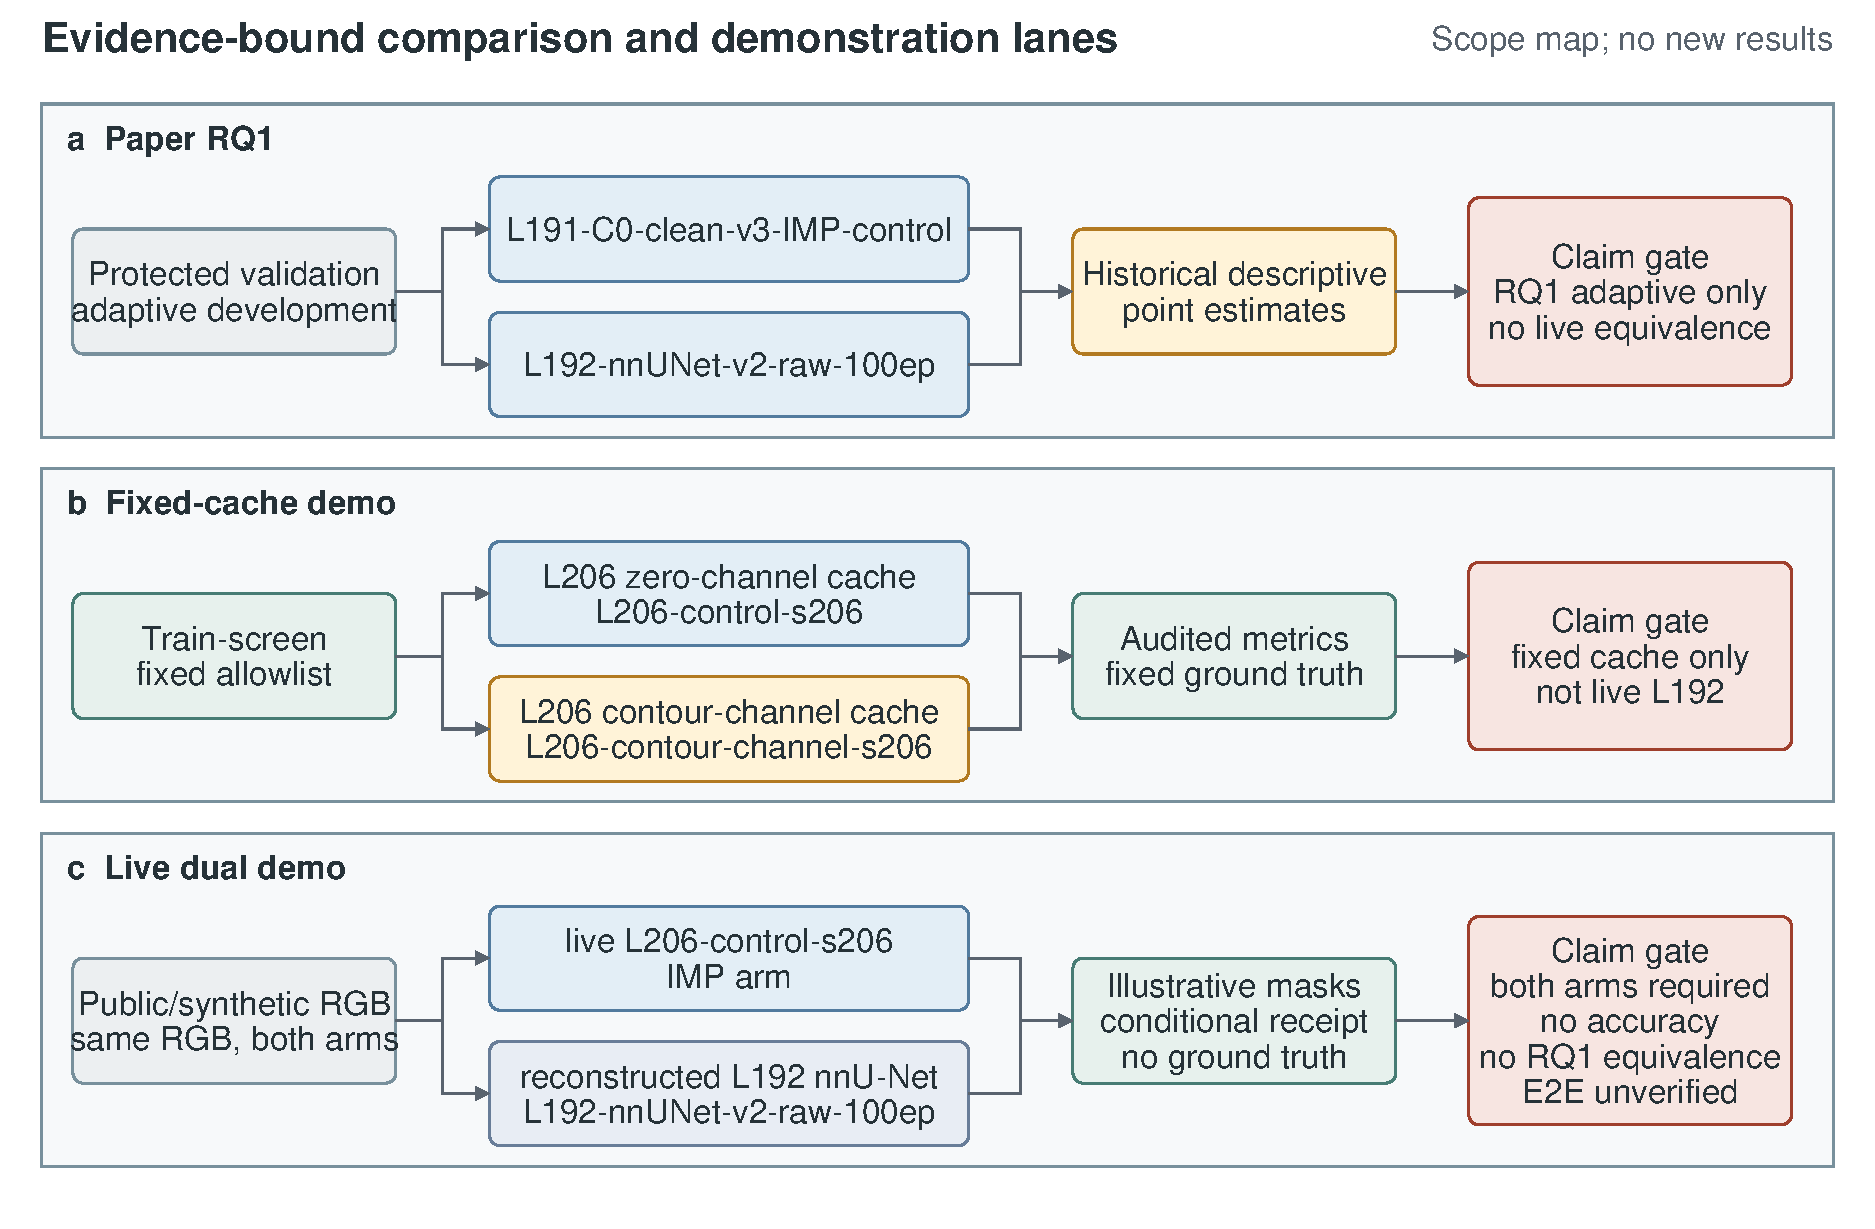
\includegraphics[width=\textwidth]{figures/evidence_pipeline.pdf}
\caption{Evidence-bound comparison and demonstration lanes. Paper RQ1, the fixed-cache demo, and the live dual demo use distinct inputs, model identities, outputs, and claim gates. Parallel arms are alternatives, not a sequential model chain. The figure supports protocol and claim-scope mapping only; it is not performance evidence.}
\label{fig:evidence-pipeline}
\end{figure*}

\subsection{Architecture comparison}

The historical Paper RQ1 comparison is L191-C0-clean-v3-IMP-control versus L192-nnUNet-v2-raw-100ep. Both use the same \cleanv{} validation identities and the six-condition robustness panel. That validation partition also informed iterative development, checkpoint or model selection, and promotion decisions, so the comparison is adaptive and potentially selection-optimistic rather than confirmatory. We report robust Dice, IoU, precision, recall, and boundary F1. Because each model has one recorded run and paired per-case evidence is not locally available in the rescue environment, no confidence interval or hypothesis test is attached to this table. Differences are descriptive point estimates.

Loop192 was evaluated against a preregistered combined promotion gate. Although its overlap and recall increased, it did not meet all boundary and precision constraints; the experiment stopped without test-v3 access. Gate failure is reported separately from metric ranking because an all-or-nothing promotion decision answers a different question from a Pareto comparison.

\subsection{Contour-channel ablation}

Loop206 uses three matched seeds. For each seed, the zero-channel control and contour-channel candidate are trained for 20 epochs on the fit portion of the 384-group train-only pilot and evaluated on the same 76 train-screen holdout groups under clean, low-contrast, and Gaussian-noise conditions. No protected image or mask participates in fitting, threshold calibration, checkpoint selection, or evaluation.

The primary endpoint is the paired candidate-minus-control robust Dice delta. Secondary endpoints include boundary F1, IoU, precision, recall, HD95, ASSD, empty predictions, and resource limits. For each split group, the procedure first averages paired candidate-minus-control deltas across the three selected seeds and three preregistered views. It then performs 10,000 paired bootstrap resamples of the 76 whole split groups. The interval preserves within-group view dependence but is conditional on the selected seeds; it does not estimate variability over seed selection.

The preregistered gate requires a positive primary effect with a positive lower confidence bound, Dice and boundary non-inferiority, clean Dice preservation, precision improvement, recall preservation, distance-metric safety, and bounded corruption regressions. Failure closes Loop206 without protected validation or test access.

\subsection{Compute}

Loop206 ran on an NVIDIA GeForce RTX 5060 Ti; preflight recorded 15.928 GiB total GPU memory. The final stage consumed 2,239.7 seconds, reached 15.644 GiB observed GPU use, 8.612 GiB process-group resident memory, and a 0.018 GiB maximum swap increase. These measurements describe the recorded run rather than a cross-platform efficiency benchmark.

\section{Results}

\subsection{Clean-v3 validation comparison}


\begin{table*}[t]
\centering
\caption{Clean-v3 validation point estimates under the older geometry contract. Both rows are single-run validation evidence; no confidence interval or protected-test result is available.}
\label{tab:clean-v3-validation}
\begin{tabular}{lrrrrr}
\toprule
Model & Robust Dice & Robust IoU & Precision & Recall & BF1 \\
\midrule
IMP-SegFormer-B3 & 0.8959 & 0.8277 & 0.9088 & 0.9128 & 0.4145 \\
nnU-Net v2 & 0.9019 & 0.8354 & 0.9056 & 0.9246 & 0.4369 \\
\bottomrule
\end{tabular}
\end{table*}


nnU-Net v2 has the higher recorded robust-Dice point estimate: 0.9019 versus 0.8959 for \impmodel{}. Its boundary F1 and recall have higher recorded point estimates, while the IMP control has slightly higher precision. These directions suggest an overlap--precision trade-off, but adaptive use of validation, the lack of repeated seeds, and unavailable paired confidence intervals prevent a statistical-superiority conclusion.

The result also does not authorize test-v3 access under the historical combined gate. The correct statement is therefore narrow: under the legacy geometry contract, nnU-Net has higher recorded \cleanv{} validation point estimates for robust Dice and boundary F1. These single-run observations are not a superiority conclusion.

\subsection{Three-seed contour-channel ablation}


\begin{table}[t]
\centering
\caption{Loop206 contour-channel minus zero-channel control on the train-screen protocol with three paired seeds, 76 groups, and 10,000 cluster-bootstrap resamples.}
\label{tab:loop206-ablation}
\begin{tabular}{lrr}
\toprule
Metric & Point delta & 95\% CI \\
\midrule
Robust Dice & -0.0313 & [-0.0491, -0.0156] \\
Boundary F1 & -0.0147 & [-0.0308, 0.0010] \\
\bottomrule
\end{tabular}
\end{table}



\begin{table*}[t]
\centering
\caption{Loop206 gate audit derived only from the hash-bound closure receipt. Every reported interval is conditional on the three selected seeds. Missing receipt fields remain \texttt{unavailable} and force \texttt{blocked} rather than reconstructing a gate decision.}
\label{tab:loop206-gate-audit}
\scriptsize
\def\sidprefix{seed-}
\resizebox{\textwidth}{!}{%
\begin{tabular}{llllllllll}
\toprule
gate\_id & endpoint & threshold & observed & interval & \sidprefix206 & \sidprefix1206 & \sidprefix2206 & status & source \\
\midrule
primary\_improvement & robust Dice delta &
unavailable & -0.0313 & [-0.0491, -0.0156] & unavailable & unavailable & unavailable & blocked & loop206\_report@7d6fcd61259a \\
dice\_noninferiority & robust Dice delta &
unavailable & -0.0313 & [-0.0491, -0.0156] & unavailable & unavailable & unavailable & blocked & loop206\_report@7d6fcd61259a \\
boundary\_noninferiority & boundary F1 delta &
unavailable & -0.0147 & [-0.0308, 0.0010] & unavailable & unavailable & unavailable & blocked & loop206\_report@7d6fcd61259a \\
clean\_dice & unavailable &
unavailable & unavailable & unavailable & unavailable & unavailable & unavailable & blocked & loop206\_report@7d6fcd61259a \\
precision & robust precision delta &
unavailable & -0.0201 & unavailable & unavailable & unavailable & unavailable & blocked & loop206\_report@7d6fcd61259a \\
recall & robust recall delta &
unavailable & -0.0142 & unavailable & unavailable & unavailable & unavailable & blocked & loop206\_report@7d6fcd61259a \\
distance & HD95 and ASSD deltas &
unavailable & 7.7911 / 5.0786 & unavailable & unavailable & unavailable & unavailable & blocked & loop206\_report@7d6fcd61259a \\
per\_corruption & unavailable &
unavailable & unavailable & unavailable & unavailable & unavailable & unavailable & blocked & loop206\_report@7d6fcd61259a \\
\bottomrule
\end{tabular}%
}
\end{table*}


\begin{figure}[t]
\centering
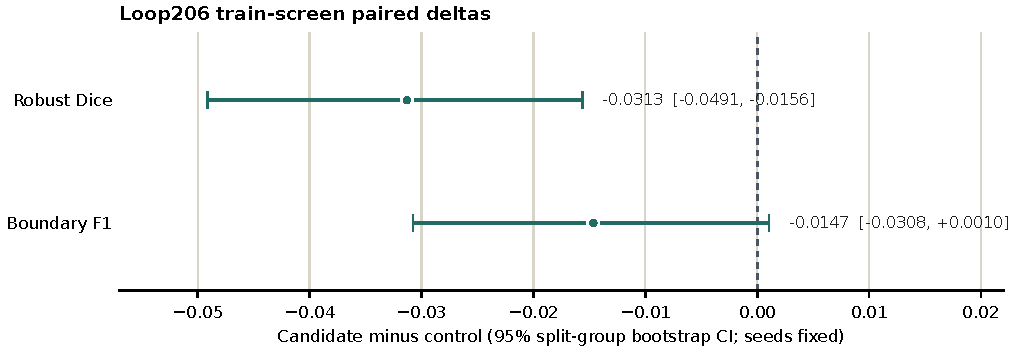
\includegraphics[width=\linewidth]{figures/loop206_delta.pdf}
\caption{Loop206 candidate-minus-control deltas on the \texttt{train\_screen} protocol with 95\% split-group cluster-bootstrap confidence intervals after averaging selected seeds and views. The intervals are conditional on those seeds. The zero line marks no paired change. Loop191 and Loop192 point estimates are excluded because paired confidence intervals are unavailable for those runs.}
\label{fig:loop206-delta}
\end{figure}

After averaging the three selected seeds and three views, the contour channel changes robust Dice by $-0.0313$. Its conditional 95\% split-group bootstrap interval, $[-0.0491,-0.0156]$, lies entirely below zero. Per-seed directions are unavailable in the authorized closure receipt, so the aggregate statement must not be read as a reduction in every seed. On this 76-group train-screen protocol, the aggregate result contradicts the stated positive primary-effect requirement; it does not establish a broader claim about contour methods or seed-population uncertainty. Boundary F1 changes by $-0.0147$; its interval $[-0.0308,0.0010]$ includes zero, providing no evidence of the intended boundary benefit. Precision and recall also decline in the recorded aggregate, while HD95 and ASSD increase.

The authorized closure receipt records only the global decision \texttt{gate\_passed=false}, establishing that at least one preregistered gate did not pass; it does not enumerate individual gate decisions. Table~\ref{tab:loop206-gate-audit} exposes the fixed eight-gate contract without reconstructing those decisions. Every interval is conditional on the selected seeds. Thresholds, per-seed directions, and unreported endpoints are \texttt{unavailable}, so every individual gate status remains \texttt{blocked}. Clean-v3 validation, test-v3, and PH2 remain sealed. The operational default and scientific reference are unchanged.

\subsection{Fixed-cache qualitative demonstration}

Figure~\ref{fig:qualitative-demo} shows three clean, non-protected examples selected without prediction or metric inspection: the first, middle, and last rows after sorting all 76 train-screen rows by sample identifier and group key. Each comparison was produced by the real GPU service and has a path-free receipt labeled \texttt{train\_screen}, \texttt{exact\_fixed\_cache}, and \texttt{historical\_cache\_provenance\_drift}. Ground truth appears only after the pinned provenance manifest verifies source identity, raw and decoded image hashes, CC-0 image license, and challenge ground-truth status. Mask bytes are separately bound to the pinned dataset index by raw, decoded-binary, and runtime digests before rendering. The panels illustrate mask geometry and disagreement; they do not estimate generalization or authorize arbitrary-upload candidate inference.

\begin{figure*}[t]
\centering
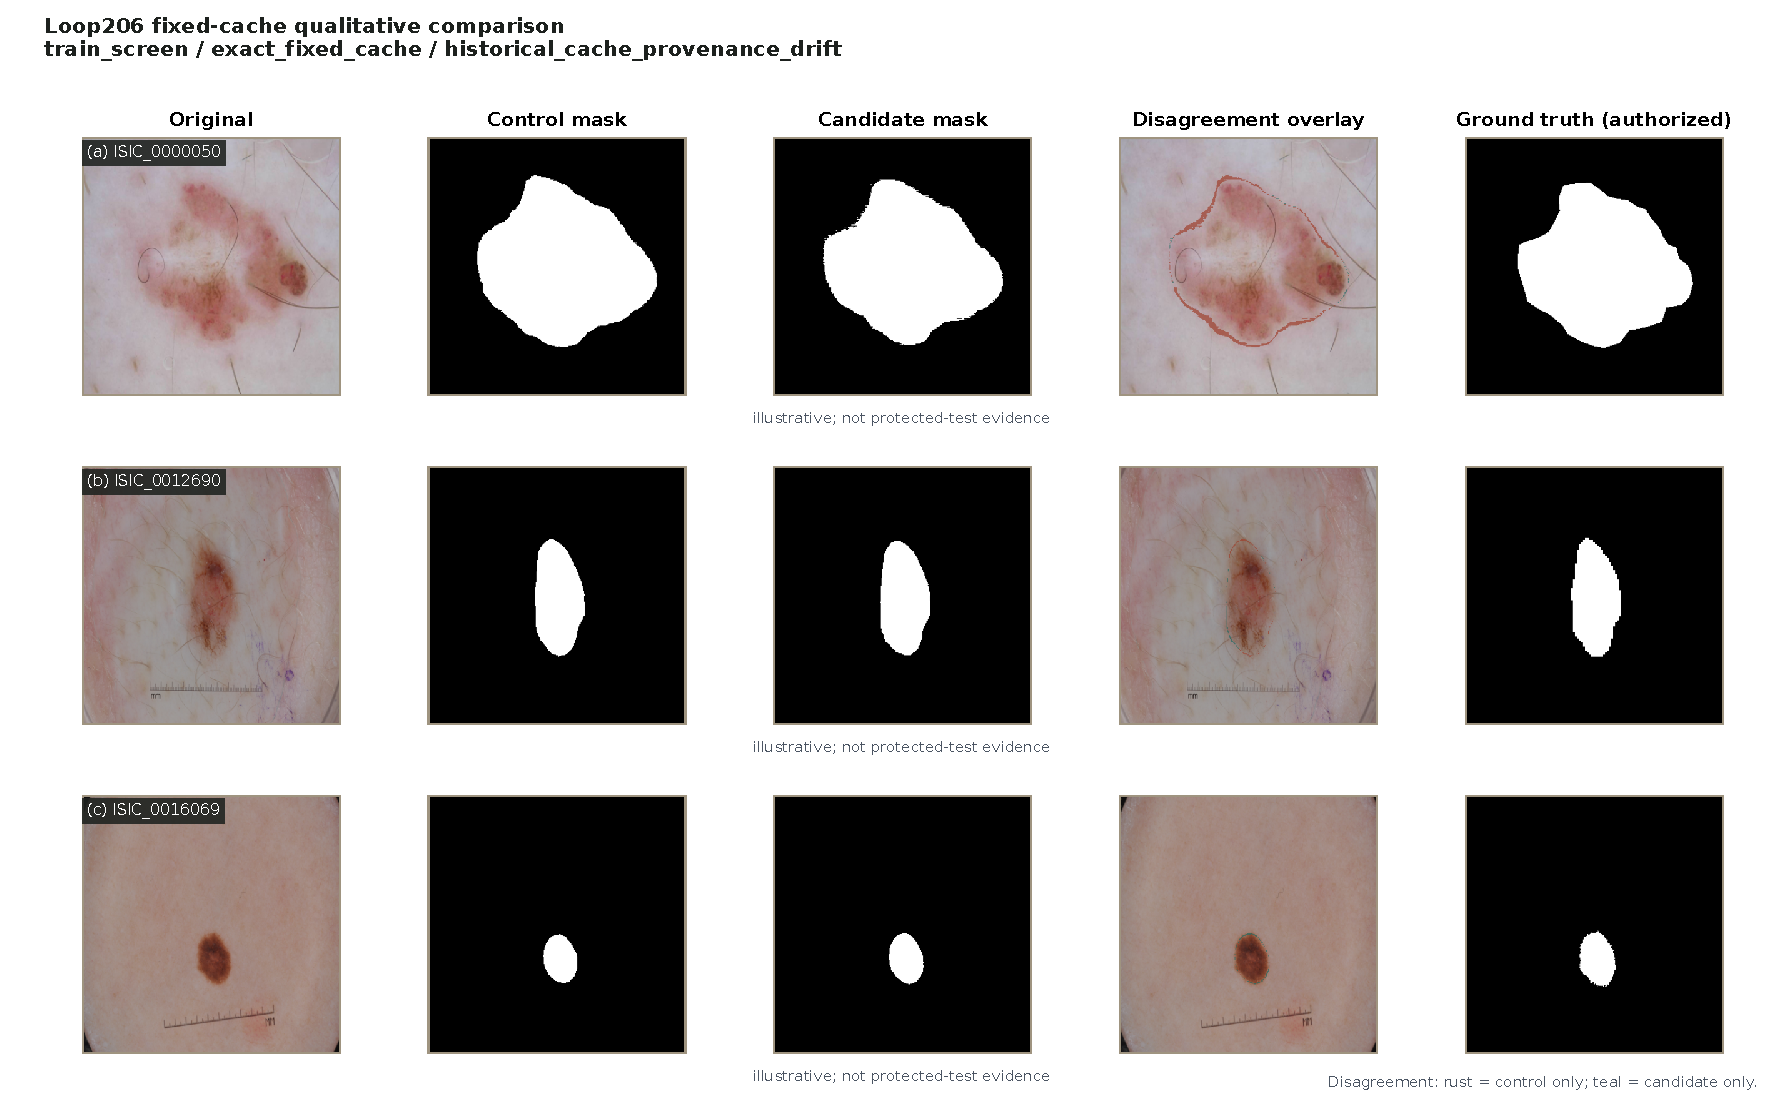
\includegraphics[width=\textwidth]{figures/qualitative_demo.pdf}
\caption{Three deterministic, non-protected fixed-cache comparisons. Columns show the original image, control mask, candidate mask, disagreement overlay, and authorized train-screen ground truth. Rust marks control-only pixels and teal marks candidate-only pixels. Each of the 15 modality subplots visibly carries the exact notice \texttt{illustrative; not protected-test evidence}.}
\label{fig:qualitative-demo}
\end{figure*}

\subsection{Bounded live dual demonstration}

Live L206-control-s206 versus a reconstructed Loop192 runtime is an illustrative, metric-free display; it does not reproduce the Loop191-versus-Loop192 Paper RQ1 comparison. In shorthand, it does not reproduce the Loop191-versus-Loop192 RQ1 comparison. The runtime is identified as L192-nnUNet-v2-raw-100ep. The service sequences independent copies of the same public or synthetic RGB input through L206 first and reconstructed L192 second; this execution order does not make either model an input to the other. A receipt is eligible only after both arms succeed and bind their model, checkpoint, input, and mask hashes. No canonical live runtime receipt is included at this stage. Ground truth is not loaded or used. Accuracy is not measured or claimed. The Live dual demo reports no metric for this live path. Its masks are illustrative.

\paragraph{Evidence classification.} Observed: the historical Task 4 resume report records bounded loopback sidecar/Gradio inference, fail-closed oversized input, retry/recovery, desktop 1440x900 and mobile 390x844 browser checks, and an ephemeral Cloudflare public GET. That historical report is not current-release acceptance evidence. Current-release browser, mobile/desktop visual, and tunnel status is \texttt{unverified/blocked}: the canonical blocked packet at \texttt{demo\_runtime/acceptance/imp.dual\_live.e2e.v1/20260722T233947051Z/acceptance.json} omits browser/tunnel fields, and the Presenter S transcript records browser discovery failure. Established: historical operational observations support only their stated checks; they do not support ground-truth accuracy or original-runtime equivalence. Assumption: no live receipt is promoted into the release, so the live lane remains separate from fixed-cache and Paper RQ1 evidence. Speculation: no causal, clinical, or superiority property follows from illustrative live masks. The historical Task 4 report recorded an 83-mask-pixel reconstructed-runtime repeat drift under matched bindings; that bounded historical observation is not current-release determinism acceptance, which remains blocked.

\subsection{Legacy comparison}


\begin{table*}[t]
\centering
\caption{Legacy Clean-v2 test-v2 values. Evidence class: \texttt{legacy\_patient\_contaminated}. Three patient IDs and 13 rows participate in cross-split contamination; these values are historical only.}
\label{tab:legacy-loop170}
\begin{tabular}{lrrrr}
\toprule
Model & Robust Dice & Clean Dice & Robust IoU & BF1 \\
\midrule
EGE-UNet & 0.8616 & 0.8617 & 0.7809 & 0.0817 \\
IMP-SegFormer-B3 & 0.8913 & 0.8962 & 0.8224 & 0.4240 \\
Vanilla SegFormer-B3 & 0.8897 & 0.8968 & 0.8179 & 0.3969 \\
nnU-Net v2 & 0.8911 & 0.8923 & 0.8246 & 0.5381 \\
\bottomrule
\end{tabular}
\end{table*}


The \texttt{legacy\_patient\_contaminated} Loop170 table demonstrates why evidence labels matter: three patient IDs and 13 rows cross split boundaries. Its point estimates would otherwise invite a direct ranking, yet this contamination violates the independence assumption required for such a claim. None of these values contributes to the main result.

\section{Discussion}

\subsection{What the architecture comparison supports}

The observed nnU-Net advantage is consistent with the value of a self-configuring biomedical pipeline, but architecture is not the only changing variable. nnU-Net uses a different resolution, augmentation policy, loss, schedule, decoder, and postprocessing path. The comparison is consequently useful as a system-level baseline: it shows that the current IMP control does not dominate a strong biomedical reference on validation. It does not identify which nnU-Net component causes the difference.

The precision direction is also important. A scalar gate that requires every metric to improve can hide a meaningful Pareto outcome, while a Dice-only ranking can hide boundary or false-positive costs. Future evaluation should report both a Dice-primary and a boundary-safe track rather than compressing all objectives into a single pass/fail label.

\subsection{Why the contour channel may fail}

The Loop206 result is more causally interpretable because the arms are matched except for the content of the fourth channel. Several mechanisms remain plausible.

First, the binary contour discards uncertainty from the regional probability map. Errors in the saliency model become sharp, high-contrast input structures that may be easier for the network to overfit than to ignore. Second, active-contour evolution is optimized as a standalone mask refinement, whereas the student network already receives RGB gradients and may not benefit from a redundant hard prior. Third, the adapter begins by ignoring the extra channel but can learn seed-specific shortcuts during a small 308-group fit. Finally, improvements observed when refining an upstream probability map do not guarantee improvements when the refined mask is used as an input feature for another learned model. The latter is a form of intervention mismatch.

The negative result does not imply that boundary information is unhelpful. It rejects a specific binary-channel mechanism. Softer uncertainty maps, auxiliary boundary supervision, native-resolution decoding, or loss-matched boundary heads remain separate hypotheses that require their own controlled experiments.

\subsection{Value of evidence repair}

The strongest contribution may be procedural. Before the audit, Loop170 appeared to provide a broad and persuasive model comparison. After patient-level review, its evidence class became \texttt{legacy\_patient\_contaminated}: three patient IDs and 13 rows cross split boundaries. The scientific default consequently changed from a model number to a status: protected-test SOTA is not established. This is a healthier outcome than preserving a favorable but contaminated claim.

\section{Limitations and Ethics}

The main architecture comparison has six substantial limitations. First, its validation partition was used adaptively for development, checkpoint or model selection, and promotion decisions, so its point estimates may be selection-optimistic. Second, it uses validation rather than protected test evidence. Third, each architecture has only one recorded run, so stochastic variance is unknown. Fourth, Loop192 probabilities were generated at $256\times256$ and resized to a $384\times384$ metric canvas under an older contract. Fifth, the compared systems differ in multiple training and architecture variables, preventing component-level causal attribution. Sixth, paired per-case predictions and the complete original dataset were unavailable in the initial Windows rescue environment, preventing metric-v2 recomputation during manuscript framing.

Loop206 improves causal control but remains a small train-screen study. It contains 76 held-out training groups, three selected seeds, and three corruption conditions. The bootstrap resamples groups after averaging those seeds and views; it does not estimate variability over alternative seed selections. Its confidence interval supports rejection of the tested contour channel on this protocol, not universal rejection of active contours, saliency, or fourth-channel models. The protected validation, test-v3, and PH2 cohorts were intentionally not opened after failure.

The live lane has historical/superseded Task 4 operational observations: sidecar/Gradio inference, desktop and mobile browser checks, fail-closed oversized input, retry/recovery, and an ephemeral Cloudflare public GET. The current canonical Task 4 browser/mobile/Cloudflare packet remains \texttt{unverified/blocked}; these bounded historical observations are not current-release acceptance evidence and do not establish end-to-end acceptance. It remains illustrative only: it has no ground truth, accuracy evaluation, canonical release receipt, or original-runtime equivalence evidence. In addition, one bundled public sample exceeds the pinned 16 MiB request contract. Repeated reconstructed nnU-Net inference drifted despite matched bindings, so determinism remains blocked. The recorded ordered shutdown closed the owned ports but exited 5; browser, tunnel, shutdown, and determinism observations do not promote a scientific result.

The source datasets are dermoscopic image collections governed by their respective ISIC challenge terms. Code and derived evidence can be shared subject to review, but raw data and model weights are not redistributed in the repository. Uploaded website images are processed ephemerally and are not retained in logs. The demonstration produces segmentation masks, not diagnoses. It has not undergone prospective, subgroup, fairness, calibration, security, or clinical validation and must not be used for medical decisions.

\section{Reproducibility}

The rescue package binds results to a canonical JSON evidence registry. Each source report is identified by a project-relative path and SHA-256. The registry records dataset version, partition, evidence class, metric contract, seed count, values, confidence intervals, and limitations. Paper tables are generated from that registry rather than transcribed manually.

The repository includes the Loop191, Loop192, and Loop206 configs; model constructors; preprocessing and postprocessing implementations; metric code; Loop205 regional saliency protocol; Loop206 active-contour implementation; evidence builder; table builder; tests; and website source. Runtime data, checkpoints, probability caches, and large artifacts remain outside Git. The selected Loop206 control and candidate checkpoints are verified by SHA-256 at application startup.

For arbitrary uploaded images, the candidate model requires a deployment saliency prior fitted only from the 308 Loop206 fit groups. Deployment is authorized only if the resulting contour generator reproduces all 76 frozen holdout clean contours byte-for-byte. If data identity, source hashes, model hashes, or contour parity fail, candidate upload inference remains disabled rather than using an approximate channel.

The recorded hardware is an RTX 5060 Ti workstation with Python 3.12. Environment dependencies are locked with \texttt{uv}. A second Windows laptop performs clean-clone CPU tests and LaTeX compilation without datasets or weights. The final release records test, paper-audit, PDF-build, GPU-smoke, and public-tunnel receipts.

\section{Conclusion}

This report replaces an ambiguous internal leaderboard with an evidence-scoped study. On the recorded \cleanv{} validation protocol, nnU-Net v2 has higher robust-Dice and boundary-F1 point estimates than the IMP MiT-B3 U-Net control, but the comparison is single-run, geometry-limited, and not protected-test evidence. In the stronger causal experiment, the three-seed Loop206 contour channel reduces robust Dice by 0.0313 with a confidence interval entirely below zero and provides no demonstrated boundary-F1 gain. The candidate is therefore rejected without opening protected partitions.

The scientifically defensible conclusion is not that a new state of the art was achieved. Under the legacy geometry contract, nnU-Net has higher recorded validation point estimates for robust Dice and boundary F1, while the tested hard contour prior fails its preregistered train-screen gate. The registry status is \verb|scientific_sota_status = not_established|. Future work should first reproduce both architectures under one original-geometry metric contract with multiple seeds, then test one boundary mechanism at a time.


\bibliographystyle{plainnat}
\bibliography{references}

\end{document}
